
\cleardoublepage

\chapter{Post-Processing Pipeline}
\label{chapter:pipeline}

Once the images are collected they must be converted into a field map. This task is accomplished by a set of scripts that are run in a sequential, or pipeline, fashion, where the output of one script is used as the input to the next.  This chapter provides a general overview of the pipeline followed by a detailed explanation of each step.

\section{Pipeline Overview}
\label{processing-overview}

In this pipeline each script is referred to as a stage, where each stage accomplishes one specific task.  The main reason the post-processing is split into separate stages is several stages take a significant amount of time to run, so it's beneficial to not re-run the entire pipeline when changes are made to one stage.  That task that each stage accomplishes is:

\begin{description}
\item[Stage 0] Calculate the position and orientation of each image.
\item[Stage 1] Find and read QR codes in all images.
\item[Stage 2] Create the structure of the field using the QR codes.
\item[Stage 3] Detect leaves and plant markers in each image.
\item[Stage 4] Cluster plant parts from stage 3 into possible plants, and filter out unlikely plants.
\item[Stage 5] Assign individual numbers to plants and save final field map to a file. 
\end{description}

The two stages that take the most time to run are 1 and 3 as they both deal with opening each image and searching through it.  Even though it would speed up the pipeline to combine them, they are kept as separate stages for simplicity.
 
The output of each intermediate stage consists of objects which directly relate to the field, for example QR codes, plants, or rows.  These objects are serialized into a single output file, which makes it trivial to pass these objects from one script to another. 

Every stage of the pipeline is written in the Python programming language, and all of the image-processing algorithms are performed using the Open Source Computer Vision library, also known as OpenCV.  The location of the post-processing code is listed in Appendix \ref{appendix:code_repositories}.

\section{Stage 0 - Calculating Camera State}
\label{processing-stage0}

The first step in the post-processing pipeline is to calculate the camera's position and orientation when each image was taken, referred to as the camera's state.  This is performed by the data collection program, since it is a general process that's useful for many other types of sensors in addition to cameras.  

However, the format of the camera position is in latitude, longitude, altitude, and the format of the orientation is Euler angles.  Therefore, this initial stage must convert the camera position to the modified \ac{utm} coordinates discussed in \ref{section:utm}, as well as calculate the homography matrix defined by equation \ref{equation:homography}.  

Even though the modified \ac{utm} coordinates use the ground reference for the z-component, the height above the ellipsoid is also tracked for each image and item mapped in the field.  This information could be used to estimate relative differences in water content in different parts of the field due to changes in elevation. 

\section{Stage 1 - Extracting QR Codes}
\label{processing-stage1}

The first goal after calculating the position and orientation of each image is to detect and read all QR codes in the image set.  This process consists of four steps which are applied to every image.

\subsection{Converting Color-Spaces}

The first step is to convert the image from the default OpenCV color-space, which is \ac{bgr}, to the \ac{hsv} color space.  As can be seen in figure \ref{figure:color_spaces}, this is a cylindrical coordinate system which separates image intensity from the color information which makes it more robust to changes in lighting. This \ac{hsv} color space is also more aligned to how humans think about color TODO insert reference.

\begin{figure}[htb]
	\centering
    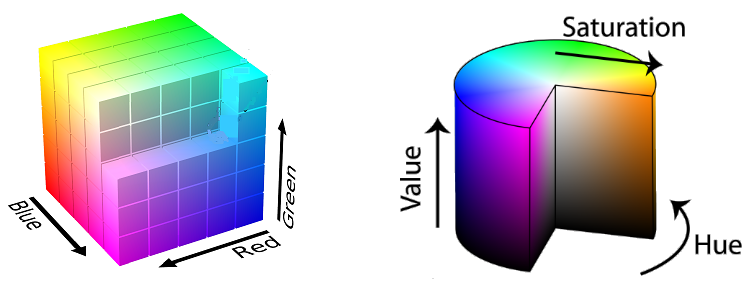
\includegraphics[width=5.5in]{figures/bgr_and_hsv.png}
    \caption[Color spaces]{Visualization of \ac{(bgr)} (left) and \ac{hsv} (right) color spaces.}
    \label{figure:color_spaces}
\end{figure} 

An important consideration is that most digital cameras perform a gamma-encoding when processing data from the imaging sensor.  This is a non-linear operation which maximizes the amount of intensity information that can be stored for each pixel, as it pertains to human-perception.  However, human perception is not a valid concern in this post-processing, and these non-linearities should be removed.  This was not realized until after the research was completed, and thus it is not implemented in the pipeline.

\subsection{Thresholding}
\label{section:qr_thresholding}

The second step is to separate the white QR code from the rest of the image.  This is accomplished by applying a range threshold for each of the HSV components.  This threshold will output a 1 (white pixel) if the all 3 components are in the specified range, otherwise it will output a 0 (black pixel).  In OpenCV hue is defined in the range of 0 to 179, and both saturation and value have a range of 0 to 255.  The range that was experimentally determined for separating QR codes is shown in table \ref{table:qr_hsv_ranges}.

\begin{table}[htb]
    \begin{center}
    \caption[QR Code Detection Values]{HSV range for detecting QR codes.}
    \begin{tabular}[c]{|c|c|c|c|}
        \hline
        Component & Min Value & Max Value & Notes \\
        \hline
        Hue        & 0   & 179 & Include all colors      \\
        Saturation & 0   & 65  & Avoid saturated colors  \\
        Value      & 160 & 255 & Avoid dark colors       \\
        \hline
    \end{tabular}
    \label{table:qr_hsv_ranges}
   \end{center}
\end{table}

This threshold results in a binary image where pixels that are mostly white, such as QR codes, are all white, and everything else is all black.  An example of a thresholded image can be seen in figure (TODO ref)

\subsection{Filtering by Bounding Boxes}

The third step is finding the set of external contours, or outermost edges, of each object in the binary image.  Each set of contours is then assigned a minimum bounding box, which is the smallest rotated rectangle that encompasses the entire object.  These bounding boxes are filtered to remove ones that are either too small or too large to be QR codes.  For the codes constructed from pot labels 

TODO include image showing original and thresholded with rotated bounding box. 

\subsection{Reading QR Codes}
\label{section:reading_codes}

The final step is to use these bounding boxes to extract parts of the original to run through the QR reading program.  From the researcher's experience the ZBar open-source program provided the best results.  However, the ZBar program requires a grayscale or binary image, and thus a threshold must be applied to the small, extracted color image.  The range threshold discussed in section \ref{section:qr_thresholding} is effective for finding possible QR codes, but does not do a good job maintaining the grid of white and black squares that make up the QR code.  Instead the \ac{bgr} image is converted to grayscale and if a simple global threshold does not result in a successful code read, then an adaptive threshold is tried instead.  This results in a readable code even if there is noticeable image glare as seen in figure TODO. 

\begin{figure}[htb]
	\centering
    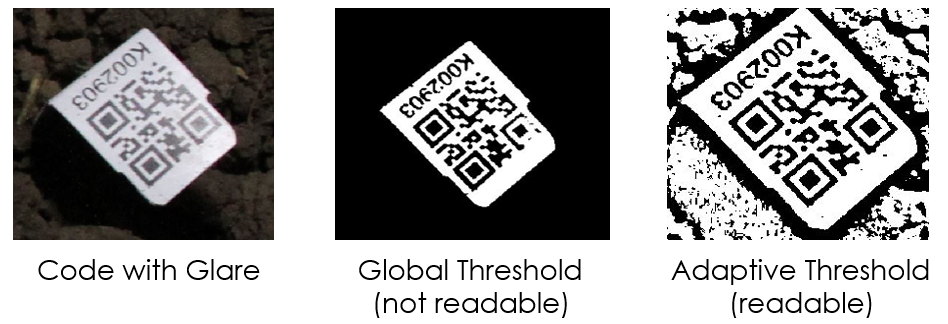
\includegraphics[width=5.5in]{figures/adaptive_threshold.png}
    \caption[Adaptive threshold]{Comparison showing how an adaptive, rather than a global, threshold can make a code readable by keeping the bottom right corner intact.}
    \label{figure:adaptive_threshold}
\end{figure} 

The data returned by the ZBar library is used to determine if the code corresponds to a plant group or to the start/end of a row.  If no data, or bad data, is returned by the ZBar library the extracted image is saved for the operator to review after the stage has completed.  This makes it much easier to find misread or damaged codes and to manually add them into the final results.  If the code is read successfully, then its world coordinates are calculated and saved in a list of QR codes.   If the same code is detected in multiple images, then the world coordinates of each reference are averaged to improve the mapping accuracy.

\section{Stage 2 - Creating Field Structure}
\label{processing-stage2}

The second stage of the pipeline involves assigning row numbers to each QR code and then creating plant groups that can span multiple rows.  As an optional input to this stage, the user can specify a file containing any QR codes from the previous stage that weren't automatically detected.  

\subsection{Assigning Codes to Rows}

This stage begins by pairing the start and end QR code associated with each row.  Since the locations of the codes are calculated from the images, the average row heading can be calculated.  This row heading is then used to transform the \ac{utm} coordinates into the field coordinate frame discussed in section \ref{section:field_coordinates}.

The next step is to assign each group QR code to a specific row based on its field coordinates.  As some rows can span several hundred meters, it's not always possible to assign a QR code to the nearest row defined by a vector between the row start and end codes.  Instead a sweeping algorithm is used.   The idea is to sweep across the field, from left to right, and incrementally add QR codes to each row as shown in figure \ref{figure:sweeping_algorithm}. Once a code is added to a row it splits that row into smaller segments.  A code is assigned to the row which has the closest segment based on lateral distance to the code's field location. 

\begin{figure}[htb]
	\centering
    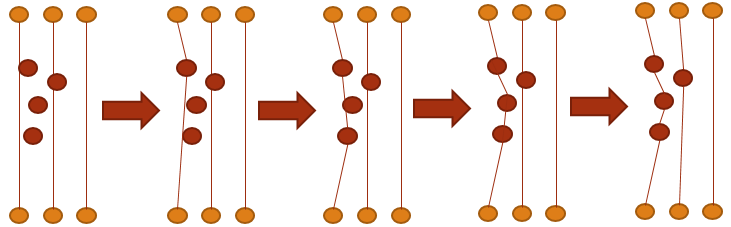
\includegraphics[width=6in]{figures/sweeping_algorithm.png}
    \caption[Sweeping projection algorithm]{Example of the sweeping projection algorithm. Row codes are shown in orange and four group codes in red.  At each step the left-most group code is assigned to the nearest segment, shown as a red line.  The result is three codes belong to the left row, and the fourth group code belongs to the middle row.}
    \label{figure:sweeping_algorithm}
\end{figure}

This algorithm can effectively account for small amounts of curvature in the rows, but is not designed to work on rows that are not planted straight to begin with.

\subsection{Organizing Group Segments}

Once all group codes are assigned to a row, it's possible to tell which codes come before and after one another.  A group segment is defined by a beginning code and the next code that follows it in the direction of planting.  This group segment is where the plants for a given code are located.  However, it's possible that when the transplanter reaches the end of a row the current plant group isn't finished and continues into the next pass.  A pass refers to the transplanter driving once down the field, so a 2-row transplanter would have a pass containing 2 rows.  Therefore, the group segments at the end of corresponding are paired together into complete groups, which is shown in figure \ref{figure:group_segments}.

\begin{figure}[htb]
	\centering
    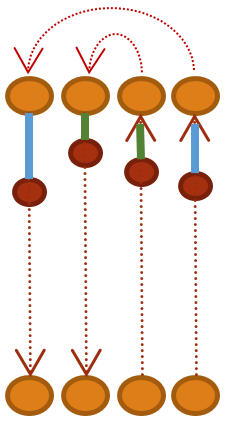
\includegraphics[height=2in]{figures/group_segments.png}
    \caption[Group segments]{Example of four rows planted two rows at a time.  The red dashed arrows show the direction of planting.  There are four group segments, two blue and two green.  The blue segments belong to the same plant group, and the green segments belong to a second plant group.}
    \label{figure:group_segments}
\end{figure}

\section{Stage 3 - Extracting Plant Parts}
\label{processing-stage3}

Similar to the process of extracting QR codes, this stage converts each image to the \ac{hsv} color space, applies a range threshold, and filters the objects based on size.  Since this stage is looking for plant leaves rather than white QR codes it uses different ranges for the HSV components, which are displayed in table \ref{table:plant_leaves_hsv_ranges}.  

\begin{table}[htb]
    \begin{center}
    \caption[Plant Leaf Detection Values]{HSV range for detecting plant leaves.}
    \begin{tabular}[c]{|c|c|c|c|}
        \hline
        Component & Min Value & Max Value & Notes \\
        \hline
        Hue        & 35  & 90  & Include green hues        \\
        Saturation & 80  & 255 & Include saturated colors  \\
        Value      & 20  & 255 & Avoid very dark colors    \\
        \hline
    \end{tabular}
    \label{table:plant_leaves_hsv_ranges}
   \end{center}
\end{table}

In addition to plant leaves, this stage also searches for plant markers.  The values for the two types of markers discussed in section \ref{section:plant_markers} are shown in the tables below.  The minimum saturation and value for the tag markers can be set much higher than the wooden blue sticks, which leads to more reliable detection.   

\begin{table}[hb]
    \begin{center}
    \caption[Blue Stick Detection Values]{HSV range for detecting blue stick markers.}
    \begin{tabular}[c]{|c|c|c|c|}
        \hline
        Component & Min Value & Max Value & Notes \\
        \hline
        Hue        & 90  & 130 & Include blue hues        \\
        Saturation & 31  & 255 & Include saturated colors  \\
        Value      & 16  & 255 & Avoid very dark colors    \\
        \hline
    \end{tabular}
    \label{table:stick_hsv_ranges}
   \end{center}
\end{table}

\begin{table}[hb]
    \begin{center}
    \caption[Yellow Tags Detection Values]{HSV range for detecting yellow tags.}
    \begin{tabular}[c]{|c|c|c|c|}
        \hline
        Component & Min Value & Max Value & Notes \\
        \hline
        Hue        & 15  & 45  & Include yellow hues       \\
        Saturation & 130 & 255 & Include saturated colors  \\
        Value      & 100 & 255 & Avoid dark colors         \\
        \hline
    \end{tabular}
    \label{table:stick_hsv_ranges}
   \end{center}
\end{table}

Similar to the QR codes these values are set based on experimentation.   However, good values for these thresholds are more likely to change due to changes in external lighting or camera settings.  This is because they depend on finding certain colors rather than white.




Besides the difference in range values this stage also adds an extra step after the threshold and before finding the contours in the image.  Then step applies two filters, the first being erosion and the second dilation.  The erosion filter removes noise from the image and the then the dilation step connects adjacent contours.  These effects can be seen in figure TODO.  The reason this step isn't used for the 

TODO maybe explain why connecting contours is a good thing.

The reason why this extra step isn't used in stage 1 is that step is already more robust based on the selected HSV range and the square nature of the QR codes doesn't benefit from connecting contours.   

\section{Stage 4 - Locating Plants}
\label{processing-stage4}

The most challenging aspect of the pipeline is reliably determining which plant parts found in the previous stage belong to the same plant, and which of those are actual plants that should be mapped.  This is challenging because there is often unavoidable plant debris in the field that comes from the tilling right before planting. TODO verify tilling word.  Plant markers, such as the blue sticks, help with this issue, but as discussed in section \ref{section:plant_localization} the blue sticks could not always be detected.  In addition, for large experiments it is not always feasible to have individual markers for every plant.  

\subsection{Hierarchical Clustering}

The task of grouping plant parts into individual plants is done using a hierarchical clustering algorithm.  In this application a cluster is represented by the minimum bounding rectangle of one or more plant parts.  If two rectangles are clustered together the resulting cluster is represented by the smallest bounding rectangle that fits both the original rectangles.  This algorithm combines the nearest two clusters into a single cluster and keeps repeating this process until an end condition is met.  The distance between two clusters is defined to be the smallest distance between any of the 4 corners of the rotated rectangles.   The end conditions are either (1) there is nothing left to cluster or (2) the closest cluster is too far apart to be clustered based on a user defined threshold.  In addition, there is a maximum size limit on the clusters, which is set to be the maximum expected plant size in the field.  Finally any tiny, unclustered plant parts are removed from the list of possible plants. 

TODO include figure showing result of clustering.

\subsection{Recursive Segment Splitting}

After the clustering is completed for an entire plant segment, the list of possible plants is passed to a recursive splitting algorithm to filter out the real plants.  This algorithm leverages information about the expected locations of plants, as well as takes into account the plant markers found in stage 3.  The splitting algorithm consists of the following steps

\begin{description}
\item[Step 1] For each possible plant, calculate the lateral and projection distance to the segment.  
\item[Step 2] Remove any plants that do not fall within the segment based on the projection distance.
\item[Step 3] Find the most likely plant based on various characteristics which is described in more detail below.  If there aren't any possible plants then create one in the next expected location based off the nominal transplanter spacing.  
\item[Step 4] Repeat the previous step, but starting at the end of the segment and find the next most likely plant by working backwards.
\item[Step 5] Split the original segment into smaller segments using the most likely plants as new endpoints.  If the new segments are too short to contain plants then the algorithm is finished, otherwise recursively go back to step 1 for each of the new segments.
\end{description}

The idea behind working from the both directions at the same time, as indicated by step 4, is the start and end QR codes are known locations in the field, and thus plants near them can be more reliably detected.  In order to determine the most likely plant in step 3, each possible plant is assigned a penalty value.  This value is calculated as

\begin{center}
Penalty = ($s_L$L + $s_P$P + $s_C$C) / ($s_B$B)
\end{center}
where those variables represent:

\begin{description}
\item[Lateral Error (L)] How far off the plant is from the expected line segment.
\item[Projection Error (P)] How far away the plant's projection onto the segment is from where the closest expected plant would be.
\item[Closeness (C)] How far away the plant is from the start/end of the segment, with the idea that the lateral and projection errors become less reliable the farther away you are from a known item's location.
\item[Plant-Part Boost (B)] Based on what types of plant parts, for example leaves or blue stick parts, are found in the plant.
\item[Scales ($s_L,s_P,s_C,s_B)$] Relative weightings to change importance of each penalty.
\end{description}

The individual penalty components are calculated with the piece-wise linear functions shown in figure \ref{figure:piecewise_penalties}.  The plant-part boost (B) is calculated as a product of additional scales for each plant part types.  If a certain type of plant part is missing from a possible plant, then its scale is set to 1 so that it has no effect.  

\begin{figure}[hb]
	\centering
    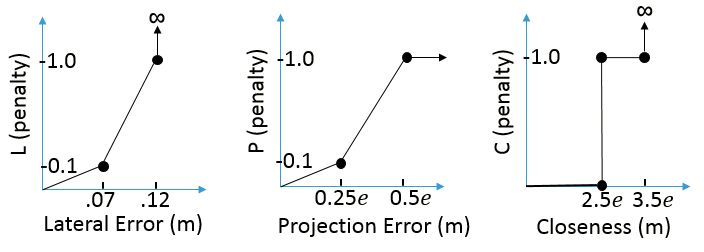
\includegraphics[width=5.5in]{figures/piece_wise.png}
    \caption[Group segments]{Piece-wise penalty functions. "$e$" represents the expected spacing between successive plants.}
    \label{figure:piecewise_penalties}
\end{figure}

The lateral and closeness penalties are defined as infinity if the input exceeds a certain threshold.  If this occurs then the overall penalty will also be set to infinity, and that plant will be removed from the list of possible plants.  If this results in no plants to select from, then a plant will be created and placed in the expected location.  These are referred to as "Created Plants", and may occur due to a plant being dead, buried, or skipped during planting.  

A simple example of the algorithm can be seen in figure \ref{figure:recursive_algorithm}.  At the beginning there is one segment between the two QR codes, which is shown in the first image.  The second image shows the result of the splitting algorithm running on segment labeled \#1. It selects one plant based on the bottom code and one based on the top code.  Segment \#2 is determined to be too short to contain more plants, however the algorithm is recursively run again on segments \#3 and \#4.  This results in the third image, which now contains five segments.  One plant had to be created because the other two possible plants on segment \#3 had too much lateral error to be considered.   

\begin{figure}[hb]
	\centering
    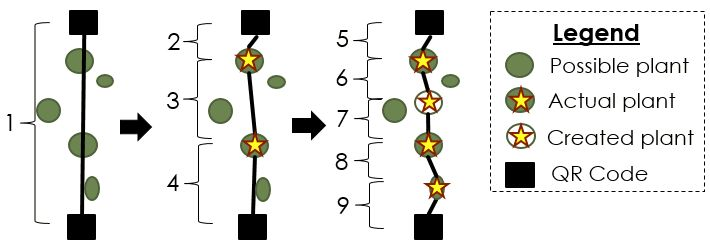
\includegraphics[width=5in]{figures/recursive_algorithm2.png}
    \caption[Recursive splitting algorithm]{Example of the recursive splitting algorithm finding most likely plants within a segment.}
    \label{figure:recursive_algorithm}
\end{figure}

Similar to the sweeping projection algorithm used to assign row numbers, this algorithm can effectively account for slight curves within a group segment since plants are incrementally determined starting at the end points. 

\section{Stage 5 - Saving Field Map}
\label{processing-stage5}

The final stage in the pipeline is generating a field map file.  This process first begins by assigning every plant in the field a unique number so it can be easily referenced in a database.  This numbering begins with plant 1 at the start of the first row, and then follows a serpentine pattern which can be seen in figure \ref{figure:serpentine}. This numbering system is chosen because it represents how a person is likely to inspect plants when walking through the field.  This numbering is done twice, once including QR codes and one just numbering plants.  After the numbering is complete, all the codes and plants are written to a \ac{csv} file, which can be imported into a database.

TODO discuss translating

\begin{figure}[hb]
	\centering
    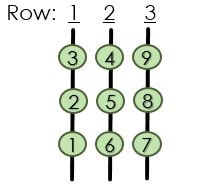
\includegraphics[height=1.7in]{figures/sepentine.png}
    \caption[Serpentine numbering]{Example of serpentine numbering.}
    \label{figure:serpentine}
\end{figure}


